\section{Evaluation of Results}\label{sec:evaluation}
We train the Neural Network model on iris data set and wine-quality data set. 

\begin{figure}[tbp]
	\centering
	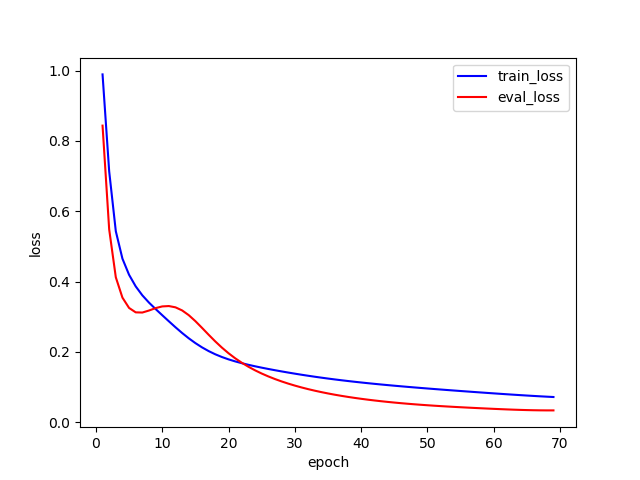
\includegraphics[width = .5\textwidth]{images/iris_loss.png}
	\caption{The epoch-loss curves for train data and validation data on iris data set.}
	\label{fig:iris_loss}
\end{figure}

\begin{figure}[tbp]
	\centering
	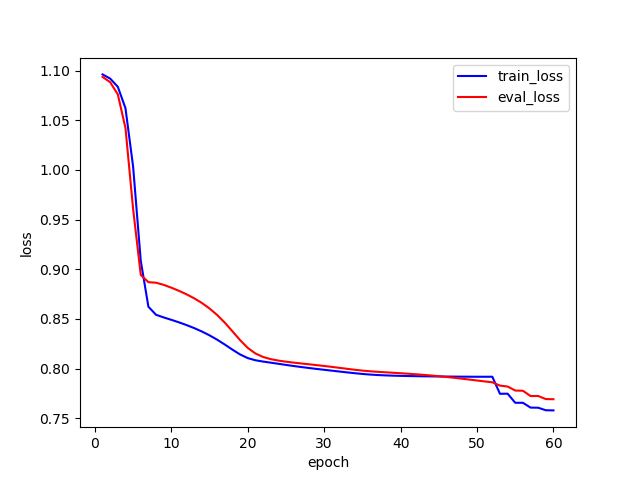
\includegraphics[width = .5\textwidth]{images/ablone-loss.png}
	\caption{The epoch-loss curves for train data and validation data on abalone data set.}
	\label{fig:wine_loss}
\end{figure}

\subsection{Accuracy Rate of Two Data Set}
For iris data set, the hidden size is 64 with one hidden layer, batch size is 8, activator is \(tanh\) and learning rate is 0.01. The curve between iterations and loss value of train data set and validation set is show as Figure \ref{fig:iris_loss}. It is early stopped after training 69 iterations. The accuracy rate of train set, validation set and test set is respectively 98.33\%, 100\% and 100\%.

For abalone data set, the hidden layers have 4 layers with 16, 32, 64 neurons, batch size is 16, activator is \(tanh\) and learning rate is 0.01. The curve between iterations and loss value of train data set and validation set is show as Figure \ref{fig:wine_loss}. It is early stopped after training 36 iterations. The accuracy rate of train set, validation set and test set is respectively 63.78\%, 62.26\% and 66.82\%.

We can see the fully connected Neural Network model performs well on nonlinear multi-classification problems, when the activator of output layer is \(softmax\) and the loss function is cross entropy. With proper depth of hidden layer and size of hidden layer, the model performs well and the accuracy is low.

However if we do not combine catalogs on abalone data set and use 29 catalogs to train the model. The accuracy is only around 25\%. Because the 29 catalogs are imbalance from which the neural network can not learn how to classify them well.

\subsection{Accuracy Rate of Different Hyper Parameters}
There are some hyper parameters affecting the performances of result, including depth of hidden layer, size of each hidden layer, batch size, activator and initialization of learnable parameters. We choose various values for each hyper parameter to evaluate the performances.

\textbf{Initialization method}. If the initial weights are full of zero. The accuracy rate on iris data is only around 50\%. The loss value decreases very slowly until number of iterations is around 500. Because when all weights are zero, the output of each layer is zero and the gradient delta of each layer is also zero except the  bias of output layer. So there is only a learnable parameter changing in the training which is the bias of the output layer. We can use random number in [-0.1, 0.1] or random number based normal distribution to initial parameters.

\textbf{Hidden layer size}. When the number of neurons of hidden layer increase, the accuracy increases first and then decreases. Because the model can not learn enough features from data set when the hidden size is too small. In comparison that, the model is easily overfitting and learn the features which is not universal but specific to this data set. So the hidden layer size should not be too big or too small.

\textbf{Batch size}.
When the bigger is the batch size from 8 to 128, the faster is the speed of each iteration. But more and more epochs are required to achieve the similar accuracy and even it can not achieve the similar accuracy, when the batch size is increasing. So the batch size should also not be too big or too small.
